 % -*- encoding: UTF8 -*-
%
%%*****************************************************************************
%%												Design & Simulation										                                        
%%*****************************************************************************

\chapter{Design \& Simulation}
\label{Ch:DesignSimulation}	

The aim of this work is to design and test a miniaturized OCT microscope as a component of a multi-modal endoscope. As described in Chapter \ref{Ch:Introduction}, this probe consist of two spectrally-separated optical paths that run partially in parallel through a micro-optical bench system. This approach allows independent tuning of the optical parameters of the two imaging modalities -- such as the NA or depth of field -- while still providing a geometrical overlap of the two acquired images. As OCT is a scanned-point imaging technique, a 2D scanning mechanism is integrated into the probe to reconstruct 3D volumes of the sample tissue.

%%*****************************************************************************
\section{Design Requirements}
%%*****************************************************************************



The OCT microscope should fulfill the following requirements:

\paragraph{Mechanical Requirements} 
\begin{itemize}

\item The scanner, electrical connections and optics should fit in a $\SI{1}{\milli\meter} \times \SI{1}{\milli\meter}$ channel. Its length should be minimized.
\item The field of view should be maximized for a 2 mm objective lens.
\item The scanning speed should be adequate for the reduced sampling rates characteristic of OCT ($\sim \SI{100}{\kilo\hertz} $).
\end{itemize}


\paragraph{Optical Requirements}

\begin{itemize}
\item The microscopy and OCT imaging fields should be coaxial to avoid parallax errors. 
\item The OCT field should be telecentric to maximize the collection of backscattered light upon normal incidence to the tissue.
\item The lateral resolution and depth of field should be adequate for OCT.
\item The backreflections inside the probe should be minimized.
\end{itemize}

  

%%*****************************************************************************
\section{Design overview}
%%*****************************************************************************

The main challenge of this work is to design a scanning mechanism compact enough to be placed in a thin, buried channel of a multimodal probe. 
Although it is theoretically possible to keep a scanner at the proximal end of the endoscope and use a coherent fiber bundle (CFB) as a relay, there are inherent drawbacks of this method, such as low light throughput, cross-talk and mechanical rigidity. 

Another challenging requirement is the superposition of the images acquired by the different modalities. If the optical axes are not coaxial, the fields will be shifted and tilted due to parallax error --- which gains importance at the small working distances common in endoscopy.

To overcome these problems, and taking into account the above-mentioned requirements, we propose a design comprising a resonant fiber scanner followed by a beam splitter, as illustrated in Figure \ref{fig:bimodalSketch}.

\begin{figure}[h!]\centering
      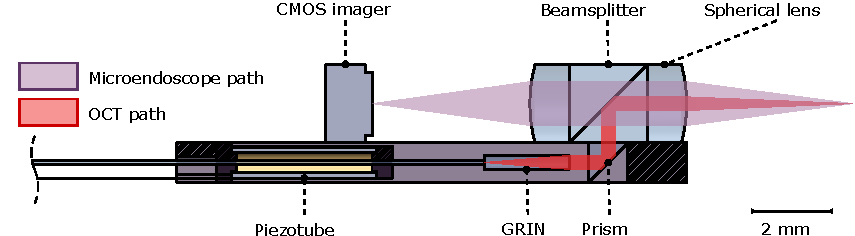
\includegraphics{figures/10_Introduction/bimodalSketch/out.pdf}
      \caption{Bimodal probe cross section showing main components and optical paths.}
      \label{fig:bimodalSketch}
\end{figure}

This implementation uses a piezo tube actuator which drives a bending beam into a resonant oscillation. This bending beam is composed of an optical fiber with a GRIN lens glued to its tip which, due to the oscillation of the fiber, radially scans a collimated laser beam. An objective lens then transforms this angular displacement into translation, as explained in Chapter \ref{Ch:Theory}. In order to merge the OCT field with the white light image, both fields are combined using a dichroic beam splitter.

There are many reasons why this design is preferred over other scanning topologies. First, the narrow dimensions of the piezo tube allow a compact implementation. Also, the field of view that can be achieved with this scanner is not limited to the space available for the GRIN lens to vibrate --- instead, to its maximum angular deflection. As we need a telecentric system, a \textit{4f} microscope could have been implemented instead of a Fourier plane scanner, but at the cost of duplicating the length of the optical system (Chapter \ref{Ch:Theory}). Finally, by gluing the GRIN lens to the tip of the fiber, its resonance frequency is greatly reduced, allowing a denser sampling.


The rest of this chapter shows the design and development of the OCT imaging path for the multi-modal probe. However, in order to independently test the behavior of the OCT scanner and optics, a single modality probe was fabricated as a demonstrator. Both systems are mechanically and optically equivalent -- the only difference is the presence of the beam splitter. 

For completeness, both multi-mode and single-mode optical systems are described.


%%*****************************************************************************
\newpage
\subsection{Optical Design}
%%*****************************************************************************

\subsubsection{Selection of Components}
\begin{figure}[h!]\centering 
\includegraphics[width=10cm,draft]{figures/foo.png}
      \caption{Fourier plane scanner indicating beam diameters, focal lengths and NAs}
      %\label{}
\end{figure}

Equations for NA, focal lengths, telecentricity

Reasons for choosing each component

\subsubsection{ZEMAX Simulation}

Table with results

\begin{figure}[h!]\centering 
\includegraphics[width=10cm,draft]{figures/foo.png}
      \caption{Layout}
      %\label{}

 
\includegraphics[width=10cm,draft]{figures/foo.png}
      \caption{Spot through focus / Field aberrations}
      %\label{}
\end{figure}

\begin{figure}[h!]\centering 
\includegraphics[width=10cm,draft]{figures/foo.png}
      \caption{Implemented 1 mode probe}
      %\label{}
\end{figure}


\subsubsection{Minimization of backreflections}
Origin of backreflections

ARC

Tilted surfaces

Position of lenses

\begin{figure}[h!]\centering 
\includegraphics[width=10cm,draft]{figures/foo.png}
      \caption{Backreflections in probe}
      %\label{}
\end{figure}



%%*****************************************************************************
\newpage
\subsection{Mechanical Design}
%%*****************************************************************************

\subsubsection{Design of the spiral scanning resonant beam}

\begin{figure}[h!]\centering 
\includegraphics[width=10cm,draft]{figures/foo.png}
      \caption{Radiant source with component sizes / Movement of spot in deltaT inside spiral}
      %\label{}
\end{figure}

Analytical calculations (res freq, bending line, max radius)

Fsampling VS FOV -> Fres, Lfiber -> +Weight, -diameter

\subsubsection{COMSOL simulation}
\begin{figure}[h!]\centering 
\includegraphics[width=10cm,draft]{figures/foo.png}
      \caption{COMSOL bending line at different voltages -> Single radiant point}
      %\label{}
\end{figure}



%%*****************************************************************************
\newpage
\subsection{Desired Design}
%%*****************************************************************************
\begin{figure}[h!]\centering 
\includegraphics[width=10cm,draft]{figures/foo.png}
      \caption{Bimodal Probe CAD render with annotations}
      %\label{}
\end{figure}


